\section{In-Database Integration}\label{sec:indatabase}
\index{data integration!in database}
As observed in Section \ref{subsec:datacleaningintegrate}, the data integration step can also be used to perform data cleaning and duplicate removal. This also implies that, when a uniform data representation for all the data sources is provided (either structured or semistructured), such data cleaning steps can be also performed within the same data model and query language \cite{deII}. It is remarked that SQL lacks a proper support for data cleaning it its 
% Given that in such representation data is structured and the support of adequate SQL operations for data cleaning is missing in  
(Commercial) Off-the-Shelf dialects: such operations must be necessarily performed at the software level, thus failing on optimizing such tasks within the same environment. 

We now outline two limitations of such language: first, SQL  does not allow  unions between tables having different schemas (\texttt{Outer Union}). This  is the first required pre-processing step before performing some further cleaning operations, as described in the incoming paragraph. This union requirement could be easily met if we change the data model and chose a semistructured representation, which is schema flexible. We start to discuss this general data model from Section \vref{sec:datamodelling}. 

Second, SQL lacks  functions clustering similar entities together (or which are able to accept collections of data collections as an input) and associating to each cluster (or data collection) one single object and -- at the same time -- preserving the original content. This is due both to data representation problems and query languages' limitations: for example, the \texttt{Group By} clause in SQL can only subsume records by aggregating them only if they share the same values for a certain set of chosen fields. For this reason, we will introduce a more general aggregation operation in Section \vref{sec:informationsintegration}.

\subsection{Preliminaries: towards a uniform data representation}\label{sec:datamodelling}
\textit{In this section we want to show that the \textsc{MetaObject Facility} (MOF) data model (used for meta-modelling) can represent different data abstraction levels}.
%\section{Preliminaries: Modelling Data}%\label{sec:preliminaries}

%In order to introduce that it exists a common representation for both structured and semistructured data, we choose to introduce the \textsc{MetaObject Facility} (MOF)\index{MOF|see{MetaObject Facility}}\index{MetaObject Facility}. Unstructured data is not mapped by any structured model, because for those data it is always required to provide to that representation some structure (see Section \vref{sec:unstructured}).

The origins of meta-modelling could be retrieved in \cite{omg96}: the OMG group aimed to develop a type system for a distributed computation system (CORBA), in order to manipulate data via ``a common, integrated set of services''. Through the definition of the \textbf{MetaObject Facility}, they wanted to distinguish between data, data collections (\textit{types}) and properties hold by such data collections. Even though it was designed for Software Engineering, such hierarchy could be also applied to database systems \cite{atzeni,encyclopedia} and the Semantic Web \cite{BrasileiroACG16}. 

\begin{definition}[MetaObject Facility]\label{def:mof}
	\index{MetaObject Facility|textbf}
The \textbf{MetaObject Facility} relies on different layers representing different abstraction (and hence, different \textbf{abstraction levels}). The first layer, simply called \textsc{Data} ($\data=D_O\cup D_R$)$\index{D|textbf}$\index{data|see{$D$}}, contains both objects\index{object} and relationships\index{relationship}. In particular, an \textbf{object}\index{object|textbf} $o\in D_O$ is an aggregation of \textbf{attributes}\index{attribute} and \textbf{values}\index{value|see{attribute}} that provides an \textit{information}. An object  composed of different objects  is referred as   \textbf{composite}. \textbf{Relationships}\index{relationship} $r\in D_R$ are n-ary association between objects. Relationships could also have a direction (\textit{directed relationships}) or not (in this case they are called ``\textit{undirected}'').

The second layer is called \textsc{Model} ($\model$)\index{model|see{$M$}}$\index{M|textbf}$ and it is a simplified representation of reality. It contains the \textbf{types}\index{type|textbf}, that are sets of objects $\mathcal T=\Set{o_1,\dots,o_n}$    satisfying a property $p$, written\footnote{Originally, \cite{omg96} used the inverse notation $p_{{T}}$, thus associating to each property a given type, and not vice versa. On the other hand, we use the notation ${T}(p)$ which resembles the notation in relational databases, where ${T}$ is the relation and the predicate $p$ is the associated schema. Moreover, in type theory \cite{TPLPierce} such relation is expressed as ${T}::p$, because both we can make correspond the types to the types in type theory, and such predicates to the sorts expressing the well-formed types.} ${T}(p)$, that is also called \textbf{schema}\index{schema|textbf} in the data science community\footnote{At this level relationships cannot be defined among types: this is one of the differences between \textsc{Model} as in the MetaObject Facility and Ontologies (Section \ref{sec:ontology}) or UML \textsc{Model} (Figure \ref{fig:umlmodelling2}).}.  Hereby, one object could belong to more than just one type (e.g.,\footnote{In this case I choose to adopt the set theory notation, widely used in relational databases to express that a tuple belongs to a relation ($t\in r$). On the other hand, in type theory an object is called a term, and to express that a term $o$ belongs to a type ${T}$ the notation $o\colon {T}$ is used \cite{TPLPierce}.} $o\in{T}_1\wedge o\in{T}_2$), and hence satisfy more than just one property.

The third layer is called \textsc{MetaModel} ($\metamodel$)\index{metamodel|see{$MM$}}$\index{MM|textbf}$, and it contains the definition of the types and of the relationships used at lower levels: in particular it contains \textbf{meta-object}s describing properties $p$ for given types \index{type}
	$\mathcal T$.
\end{definition}

Besides of the very general representation of both entities and relationships, such model   allows to point out at which abstraction level a query language must be located, thus introducing the next topic on ontologies. Moreover, its general definition of ``value'' allows it to be either an atomic value, or a collection of values, and each value could be also an object.

 \begin{sidewaysfigure}[!p]
	\centering
	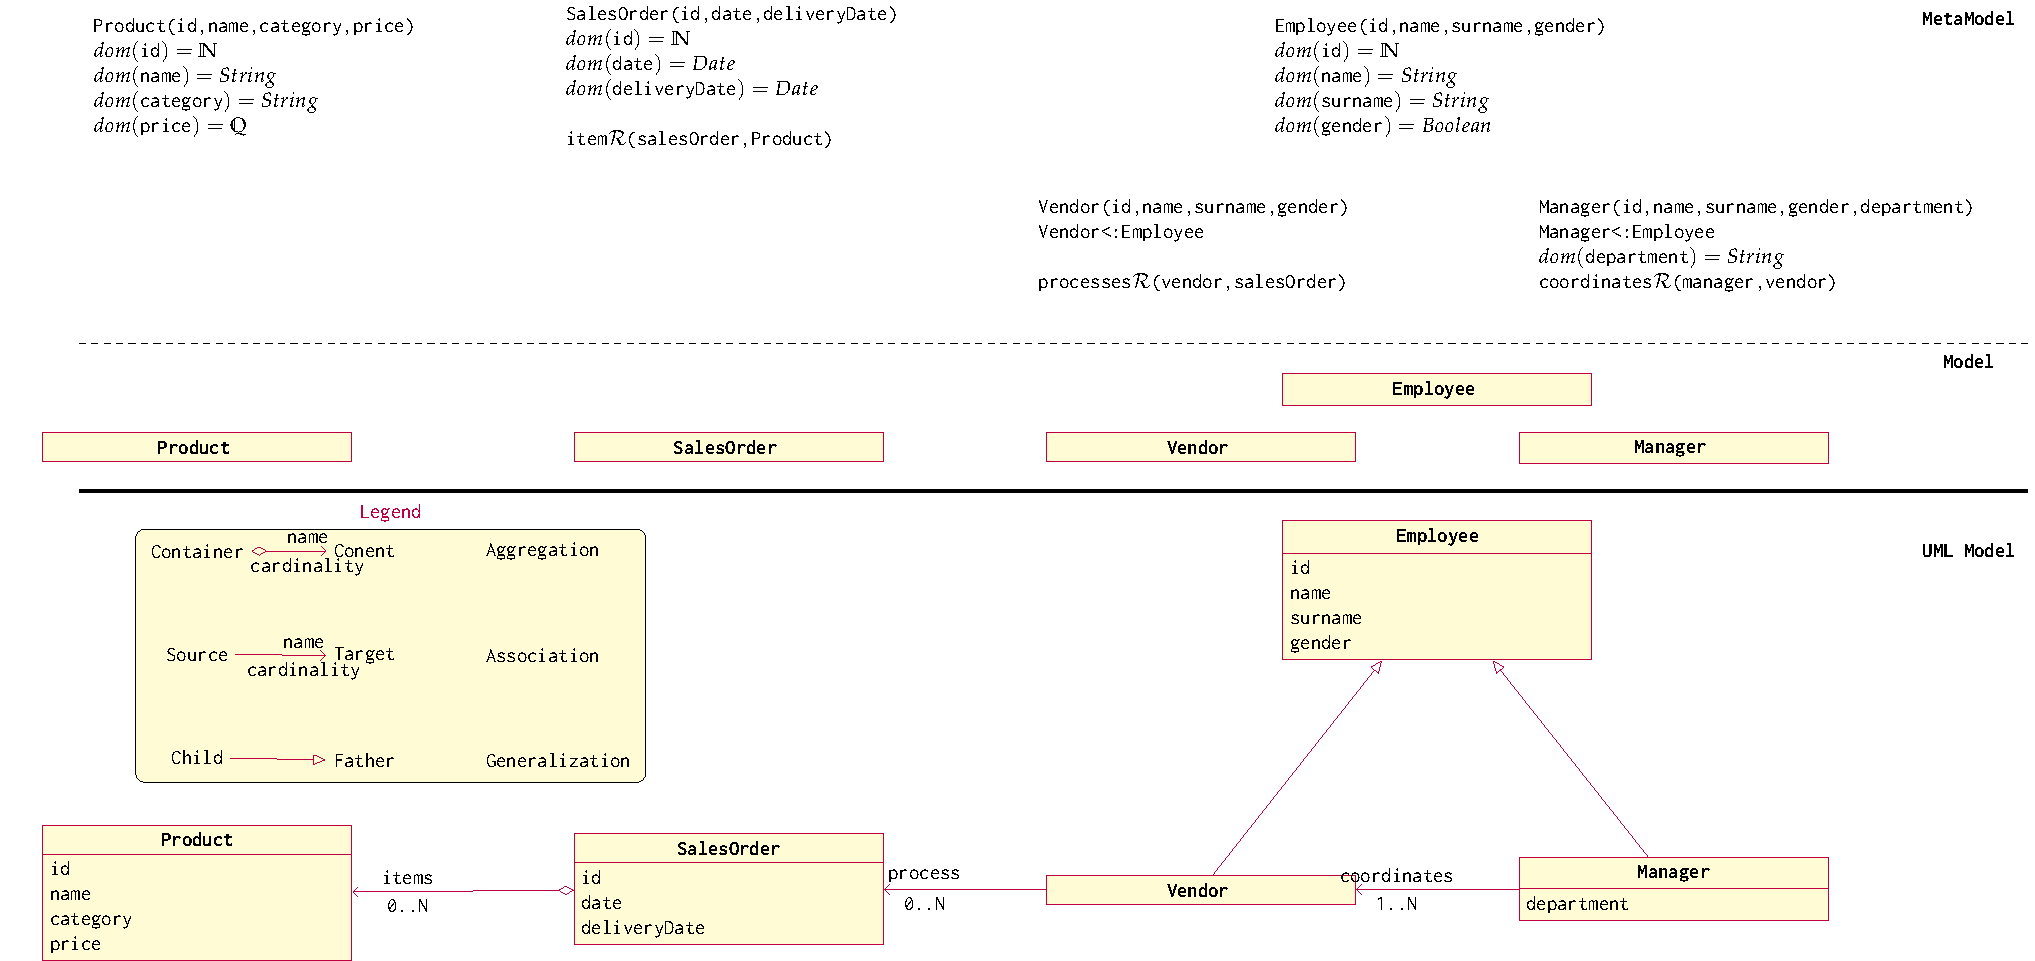
\includegraphics[width=\textheight]{fig/01dataint/umlmodelling2}
	\caption{Comparing the UML model representation and the one provided in Definition \ref{def:mof}. The white diamond represents \textbf{part-of} relations and the white arrow represent  \textbf{is-a} relations. As we could see, the UML \textsc{Model} already provides a structured notion of the types, since the type definition and the schema is not separated as in the MetaObject Facility. Hereby, we will continue to use the MetaObject Facility serparation between \textsc{Model} and \textsc{MetaModel}, thus allowing to provide a data representation which is not schema related. In particular, we use the relational data model way to provide the schema property for the types, and use the Datalog syntax for expressing relationships among types.}
	\label{fig:umlmodelling2}
\end{sidewaysfigure}

Despite the aforementioned definition, there is no universal acclaim of what a \textsc{MetaModel} should be. \cite{mathmeta} points out some alternative approaches that have been followed on this regard (e.g., for the UML modelling language \cite{OMG2011a} extending the MOF): either \begin{inlinelist}
 	\item the \textsc{MetaModel} is the modeling language itself, allowing to outline the \textsc{Model} and its instance, or
	\item The \textsc{MetaModel} is a model for the modelling language
 \end{inlinelist}. The choice of UML of class diagrams that could be used on both the \textsc{Model} and the \textsc{MetaModel} level causes a limit in the expressive power of the meta-modelling language, that could not be used to define more advanced properties (Figure \ref{fig:umlmodelling2}) and, for example, cannot lead to the definition of a query language\iffalse, contrariwise to Description Logic (see Section \ref{sec:ontology})\fi. Hereby, we will continue to use the \textsc{MetaModel} definition that was previously provided: as a consequence, \textsc{Model} and \textsc{MetaModel} do not abstract from the data structures, but characterize the properties hold by the same initial data. %As a consequence, we have that the same data level contains all the informations on how the data is structured.
\begin{sidewaysfigure}
	\centering
	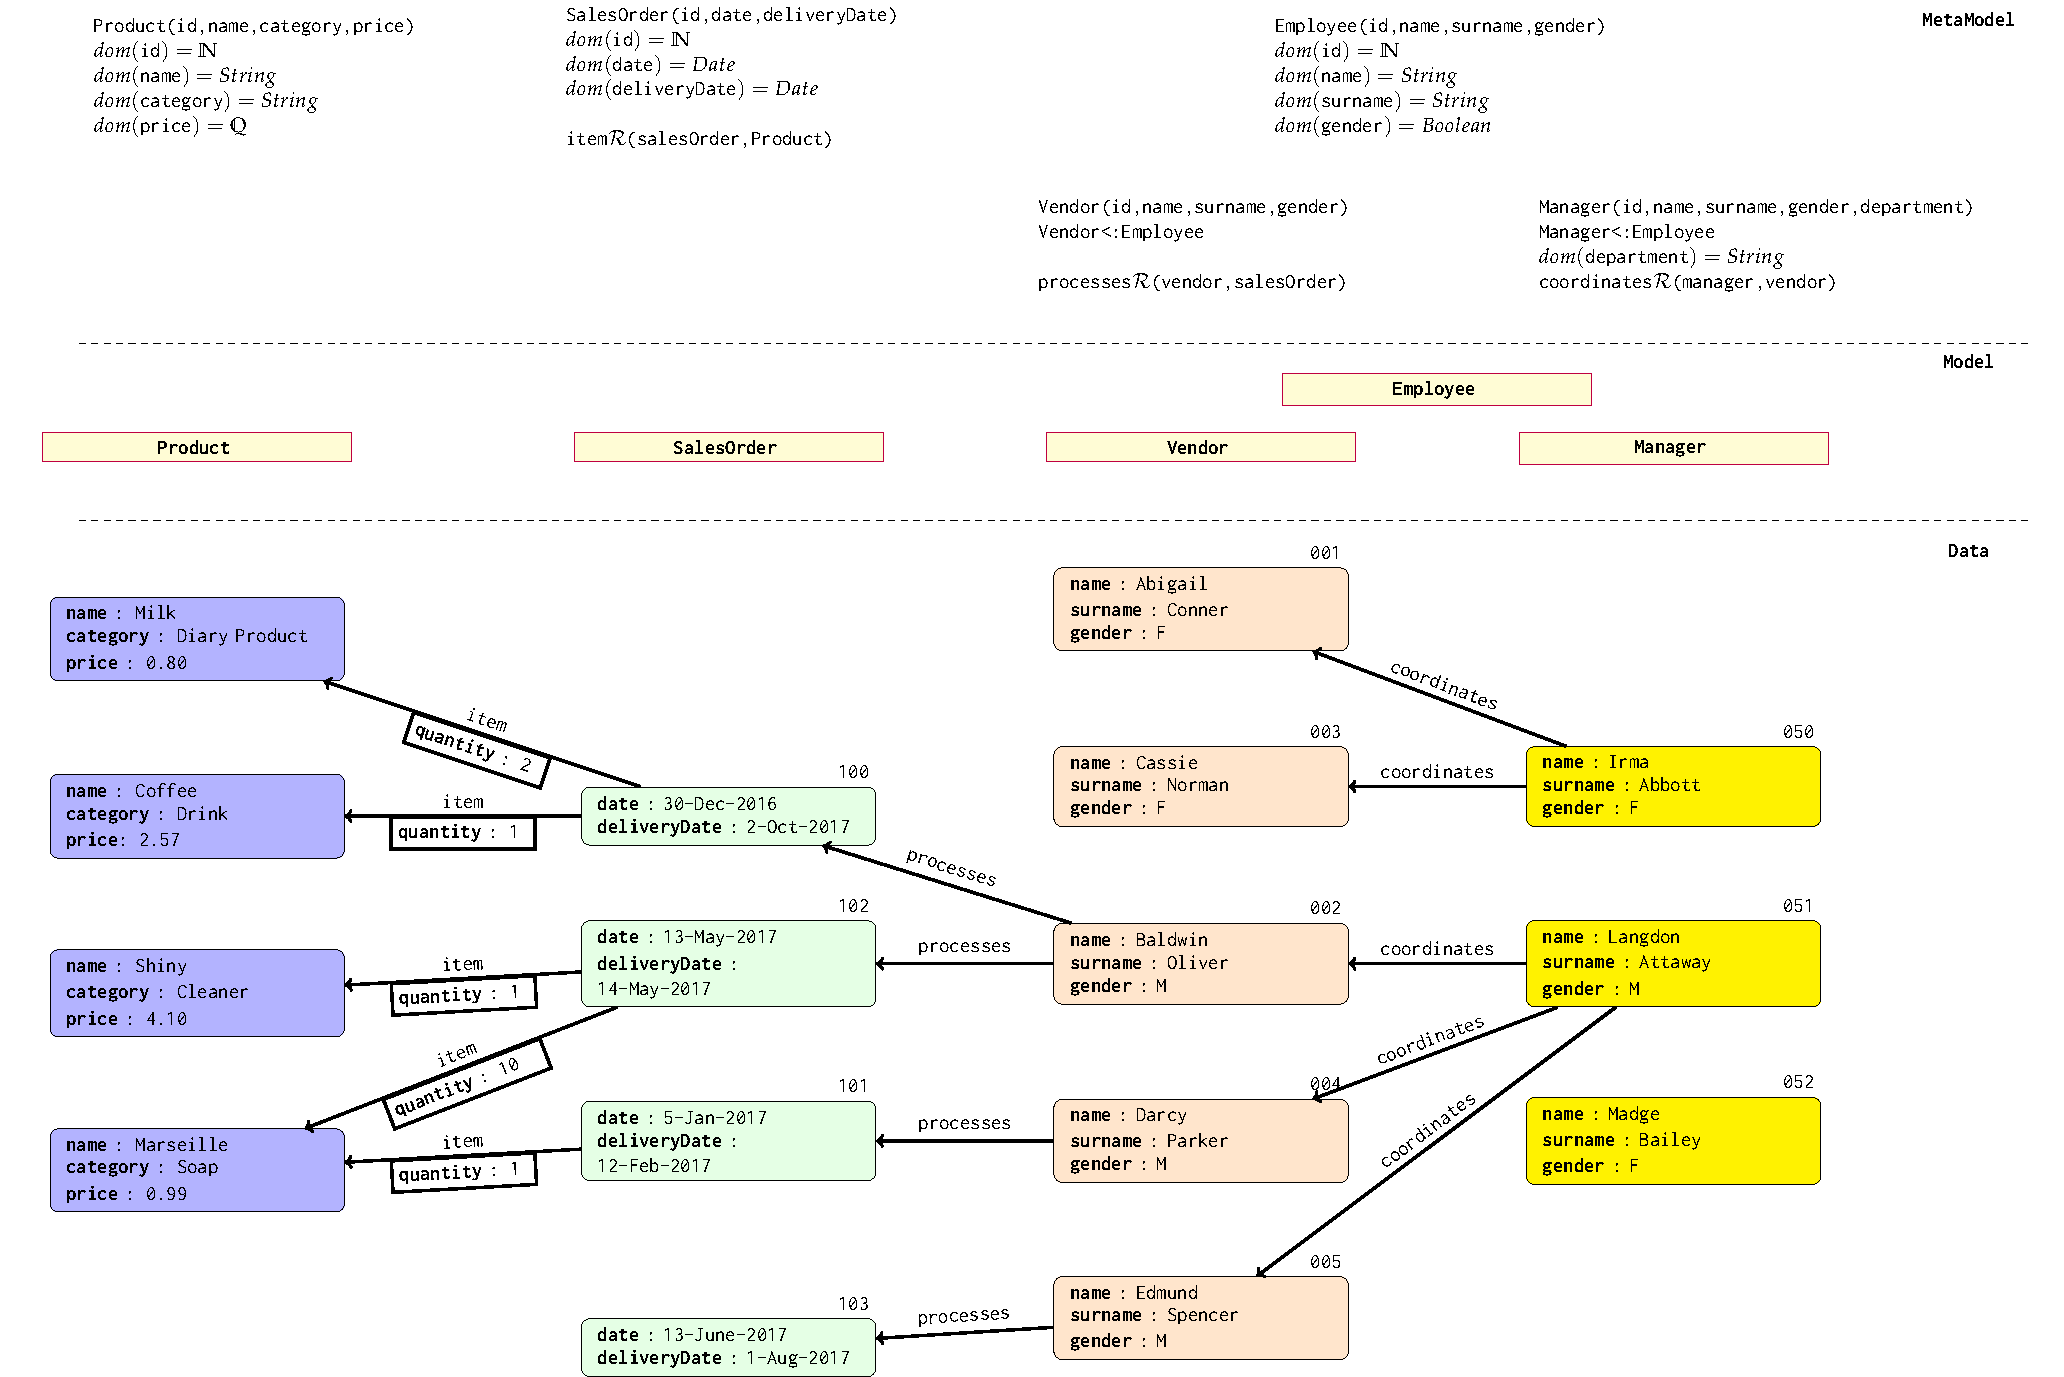
\includegraphics[width=\textheight]{fig/01dataint/umlmodelling}
	\caption{Complete MetaObject Facility example. Each object in the \textsc{Data} layer which has a given type (provided on the top label in bold) is associated to the class in the \textsc{Model} layer with an $\alpha$ relation.}
	\label{fig:umlmodelling}
\end{sidewaysfigure}

\begin{example}
	Figure \ref{fig:umlmodelling} provides an example of all the MetaObject Facility layers for a vending company use case scenario. In particular, we represent two types of \texttt{Employee}s, \texttt{Vendor}s and \texttt{Manager}s. The latter ones coordinate the former ones, while the first ones can process \texttt{SalesOrder}s order containing \texttt{Product}s. One \texttt{Manager} could \texttt{coordinate} one or more \texttt{Vendor}s, which could \texttt{process} some \texttt{SalesOrders} composed of several \texttt{items}, which are \texttt{Products}. All the objects sharing the same type are arranged in the same column where their correspoding type at the \textsc{Model} level is located, on top of which its properties at the \textsc{MetaModel} are provided.
\end{example}

As we could se from the former example, such model allows to represent a graph: each object could be considered as a vertex, while each relationship as an edge. As a result, we have that even edges must be represented as primary concepts within the  MetaObject Facility. Hereby, even each relationship should be a primary concept within this modelling definition, and hence each edge should have an associated type, as it happens in current graph databases (compare with edge \textit{labels}). On the other hand, this already happens within the UML modeling language \cite{OMG2011a, OMG2011}.

Given that the schema and all the properties pertaining to the types are expressed as properties, it is now easy to define any query \textsc{Language}\index{language|see {$\langg$}} $\langg_\metamodel$ on top of the \textsc{MetaModel} $\metamodel$ through which express the schema of the types at the \textsc{Model} level by abstracting from the data representation. The fact that $\langg_\metamodel$ includes $\metamodel$ is confirmed by the fact that \textit{queries} could be represented as mere combinations of to-be-satisfied properties, as well as schema representations \cite{Lenzerini02}. Please note that such query  \textsc{Language} ($\langg_\metamodel$) does not belong to the original MetaObject Facility model, and that it has been introduced at this level for the first time within this thesis for modeling purposes.

Between such abstraction layers only an ``instance-of''\index{instance of|see {$\alpha$}} function\footnote{$\abstr$ is a widely adopted symbol field for many different aspects: it is also a relational algebra operator for transitive closures \cite{Alpha}, one of the two possible data aggregations presented in \cite{Johnson2011} or an alignment between two ontologies \cite{euzenat2013d}.} $\alpha$ is allowed to connect  each lower layer to the  immediately upper one \cite{mathmeta}; such kind of relation is not allowed  between instances of the same layer, and hence it could not be used to provide aggregations within the \textsc{Data} layer. As a consequence, $\alpha$ should be denoted by the following expression:
\[\abstr\colon \data\cupdot \model \to \model\cupdot \metamodel\]
where $\cupdot$ provides the disjoint union between two sets, thus allowing to map each element of $D$ into one of $M$, and similarly for $M$ and $MM$. Such function is defined in literature as follows:

\begin{definition}
	An \textbf{abstraction function} is an $\abstrTHIS$  \index{abstraction|see{$\alpha$}} relation that is
	defined as follows:
	\begin{equation}\label{eq:alayer}\metamodel=\abstr(\model)=\abstr(\abstr(\data))\end{equation}

	Such $\abstr$ could be seen as the following transformation between
	objects at different layers of abstraction \cite{kuhne06a}:
	\begin{equation}\label{eq:alpha}
	\ttransl \circ\abstr'\circ\pi
	\end{equation}
	where $\pi$ is a projection function that reduces the informative content of the
	given object, $\abstr'$ provides a further abstraction (i.e.,\; over object's
	relations) and $\ttransl$\index{translation!data|see{$\ttransl$}} translates the refined object into a more abstract
	modeling language. Sometimes \cite{kuhne06a} $\abstr'$ could be omitted or
	replaced by an identity function.
\end{definition}

Since there is an unique function for abstracting different layers, this function also makes possible that each layer could be represented similarly. The possibility of doing so is also confirmed for the previously-introduced  ``semi-structured data''\footnote{See Chapter \vref{sec:semistructured} for more details.}. For the moment is only sufficient to know that the visual language UML extending the aforementioned model \cite{OMG2011,OMG2011a}, could be expressed with a (semistructured) XML specification, called XMI \cite{XMI}, through which \textsc{Data}, \textsc{Model} and \textsc{MetaModel} could be all represented. Given that XML can express both data and model layers, XML provides a better abstraction than the former model. Please also note that XML syntax can be also used to represent query languages (XSLT) and, therefore, XML may be also used to represent all data representation layers in the former model. Therefore, semistructured data provide a more uniform representation allowing the definition of $\alpha$ as simply as a XML transformation function. 


As it will be outlined in the next chapter, XML has also modelling limitations for representing nested concepts. Therefore, not even XML can be totally adopted as a suitable model for data integration. We procrastinate the discussion for our proposed Data Model to Chapter \ref{cha:graphsdef}. Bearing this in mind, we're still considering within this chapter MOF as the final data model of choice. 